\chapter{Casos de Uso}
\label{chapter:casos_de_uso}

% Escrever sobre caso de uso do sistemas
No capítulo \ref{chapter:projeto} descrevemos o funcionamento da Interface e sua comunicação com a linguagem MQTT. Este capítulo busca demonstrar o funcionamento do sistema em hardwares com a interface implementada pelos softwares descritos na seção \ref{section:codigos_fonte} disponível no Apêndice. São aplicações simples que mostram a facilidade e a escalabilidade do sistema, além de demonstrar como o sistema pode ser implementado em plataformas.

\section{Medição de temperaturas de CPU}
\label{section:temp_cpu}

Este exemplo tem como objetivo medir a temperatura da CPU de um console com baseado em suas atividades, serviços e processos em execução. A aplicação pode ser escalada para a obtenção de outras informações da CPU e do sistema, podendo assim disponibilizar análises de desempenho da plataforma, além de montar perfis de uso do sistema e administrar seu uso.

Para isso precisaremos utilizar um Publisher no console a ter informações de temperatura a ser coletadas e um Subscriber para receber estas temperaturas via MQTT e persisti-las em banco de dados. Ambas as aplicações utilizarão as APIs em Javascript, utilizando Node.js para coletar as informações do sistema, implementar o Publisher, o Subscriber, o driver para MongoDB (também disponível em anexo) e a geração de um gráfico utilizando a plataforma plotly \cite{plotly}.


\begin{figure}[h!]
\centering
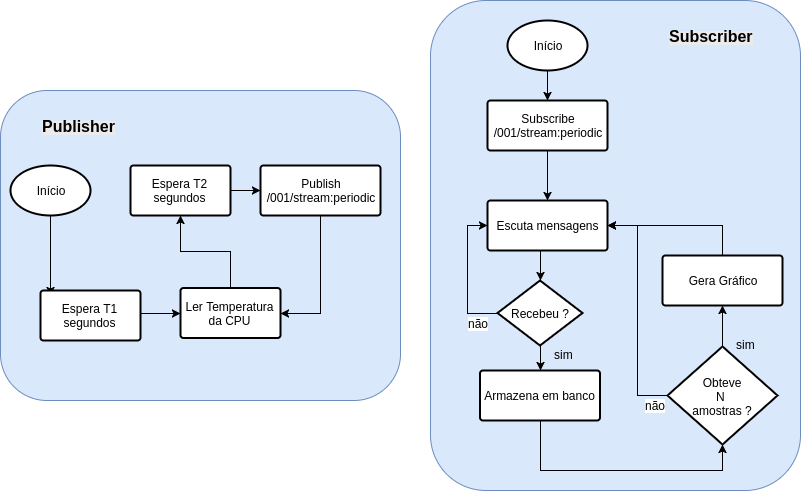
\includegraphics[width=11.5cm]{./02_Capitulos/02_Cap4/figures/fluxo_controle_temp}
\caption{Diagrama de fluxos do Publisher e do Subscriber}
\label{fig:4.1.0/fluxo_controle_temp}
\end{figure}

% Falar sobre o diagrama de fluxo
A \ref{fig:4.1.0/fluxo_controle_temp} mostra todo o fluxo das duas aplicações, o Publisher publica em no tópico \textit{/001/stream:periodic}, a informação coletada a cada T1=3 segundos e espera T2=1 antes de enviar. O Subscriber escuta este tópico e persiste ao chegar uma mensagem de dados pelo Data Stream, ao atingir N=100 amostras, um gráfico de Temperatura da CPU principal pela Data-Hora de inserção é gerado com as últimas 100 inserções no banco.


% Inserção no banco
Repare que a medição depende da data e da hora de inserção no banco, o tempo de chegada até a persistência varia muito com a latência e com o processamento da aplicação, desta forma temos uma medida mais constante. A \ref{fig:4.1.0/comapass} mostra o formato de dado armazenado, com a ferramenta Compass para visualização de dados do MongoDB. Repare que lidamos com a estrutura de dados em documento porém obrigatoriamente todo documento da Interface possui o timestamp da inserção no banco, o campo data é o objeto de dados em medição.

\begin{figure}[h!]
\centering
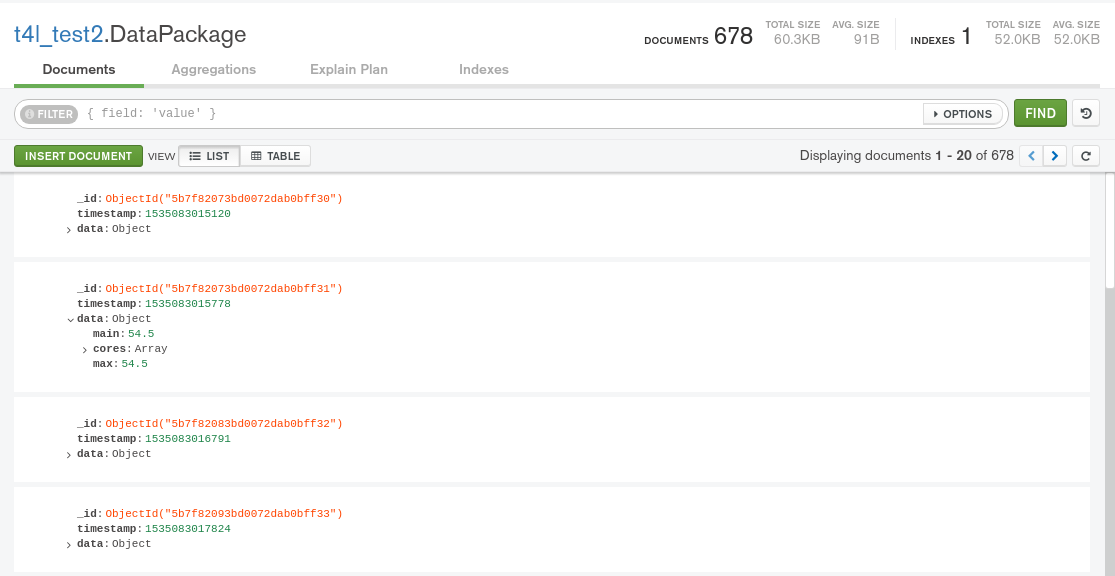
\includegraphics[width=15cm]{./02_Capitulos/02_Cap4/figures/compass}
\caption{Visualização dos dados armazenados em documento em uma coleção do MongoDB}
\label{fig:4.1.0/comapass}
\end{figure}

% Visualização com o plotly
A visualização de dados é feita pela ferramenta Plotly, um serviço que fornece uma interface para criar, editar e analisar gráficos, basta criar uma conta, gratuíta ou paga, e o usuário poderá criar gráficos na plataforma web ou através de APIs implementadas em múltiplas linguagens de programação conhecidas. A aplicação do Subscriber utiliza da segunda opção com o módulo plotly.js, a implementação em Javascript da plataforma. A cada N=100 amostras são produzidos gráficos como o da  \ref{fig:4.1.0/cpu-temp_1}.


\begin{figure}[h!]
\centering
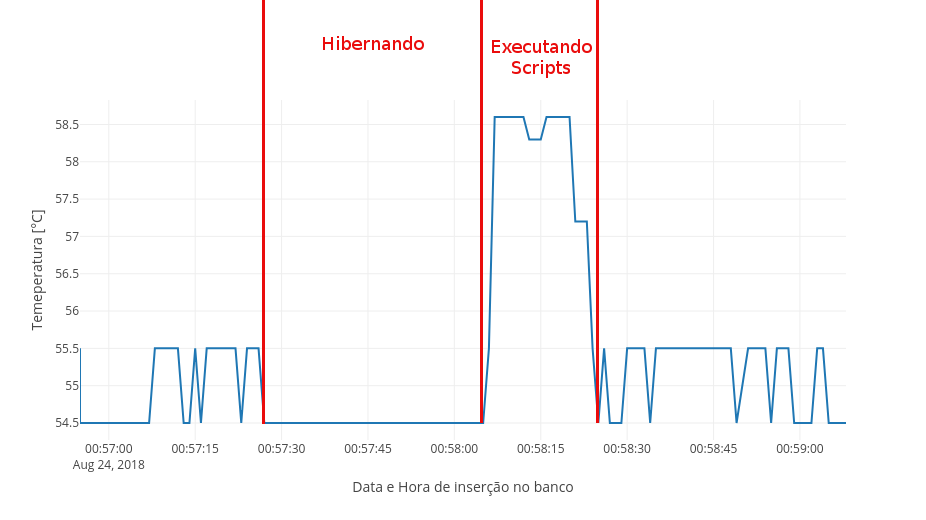
\includegraphics[width=16cm]{./02_Capitulos/02_Cap4/figures/cpu-temp_1}
\caption{Comportamento da temperatura em três momentos}
\label{fig:4.1.0/cpu-temp_1}
\end{figure}

A \ref{fig:4.1.0/cpu-temp_1} mostra a variação da temperatura de uma CPU da Intel Core I7 em três momentos. O gráfico começa no primero momento onde só os processos básicos do computador estão em execução, mantendo a temperatura constante, logo em seguida entra o momento onde o computador está hibernando o que leva a uma pequena baixa na temperatura. O terceiro momento descreve o comportamento quando o computador executa o MATLAB em um script que exige capacidade de processamento, causando uma leve alta de temperatura, mas não tão lata devido a capacidade do processador e depois estabilizando e voltando ao primeiro momento. Com isso fechando o ciclo das aplicações.

